

\documentclass[tikz, border = 0.2 cm]{standalone}
\usepackage{tikz}

\begin{document}
\noindent
\begin{tikzpicture}
\node [anchor=west] (note) at (-1,6) {%
    \begin{tabular}{@{}l@{}}
        $\alpha=-1.5$ \\
        $\mu=20$
    \end{tabular}
};
\node [anchor=west] (water) at (-1,2.5) {%
    \begin{tabular}{@{}l@{}}
        $\alpha=-2.5$ \\
        $\mu=50$
    \end{tabular}
};%{$\alpha=-2.5$,\, $\mu=50$};
\node [anchor=north] (bottom) at (8, 9.5) {$\alpha=-8$,\, $\mu=2 $};
\node [anchor=north] (bottom2) at (3.2, 9.5) { $\alpha=-6$,\, $\mu=1$};
\node [anchor=south] (top) at (3.2, -1.0) { $\alpha=-10$,\, $\mu=3$};
\node [anchor=south] (top2) at (8, -1.0) { $\alpha=-3$,\, $\mu=100$ };
\node [anchor=east] (right) at (12.3, 6) {%
\begin{tabular}{@{}l@{}}
        $\alpha=-2$ \\
        $\mu=30$
    \end{tabular}
};%{ $\alpha=-2$,\, $\mu=30$};
\node [anchor=east] (right2) at (12.3, 2.5) {%
\begin{tabular}{@{}l@{}}
        $\alpha=-20$ \\
        $\mu=4$
    \end{tabular}
};%{$\alpha=-20$,\, $\mu=4$};
\begin{scope}[xshift=1.5cm]
    \node[anchor=south west,inner sep=0] (image) at (0,0) {\includegraphics[width=0.7\textwidth]{../sim_phantom}};
    \begin{scope}[x={(image.south east)},y={(image.north west)}]        
        \draw [-latex, line width=1pt, black] (note) -- ++(0.3,0.0);
        \draw [-stealth, line width=1pt, black] (water) -- ++(0.3,0.0);
        \draw [-stealth, line width=1pt, gray] (bottom) -- ++(0,-0.2);
				\draw [-stealth, line width=1pt, gray] (bottom2) -- ++(0,-0.2);
        \draw [-stealth, line width=1pt, gray] (top) -- ++(0,0.13);
				\draw [-stealth, line width=1pt, black] (top2) -- ++(0,0.13);
        \draw [-latex, line width=1pt, black] (right) -- ++(-0.22,0);
				\draw [-latex, line width=1pt, darkgray] (right2) -- ++(-0.3,0);
    \end{scope}
\end{scope}
\end{tikzpicture}%
\end{document}


%\documentclass[tikz, border = 0.5 cm]{standalone}
%\usepackage{tikz}
%
%\begin{document}
%\noindent
%\begin{tikzpicture}
%\node [anchor=west] (note) at (-1,6) {%
    %\begin{tabular}{@{}l@{}}
        %$\alpha=-1.5$ \\
        %$\mu=20$
    %\end{tabular}
%};
%\node [anchor=west] (water) at (-2,2.5) {$\alpha=-2.5$,\, $\mu=50$};
%\node [anchor=north] (bottom) at (8, 9.5) {$\alpha=-8$,\, $\mu=2 $};
%\node [anchor=north] (bottom2) at (3.2, 9.5) { $\alpha=-6$,\, $\mu=1$};
%\node [anchor=south] (top) at (3.2, -1.0) { $\alpha=-10$,\, $\mu=3$};
%\node [anchor=south] (top2) at (8, -1.0) { $\alpha=-3$,\, $\mu=100$ };
%\node [anchor=east] (right) at (13.3, 6) { $\alpha=-2$,\, $\mu=30$};
%\node [anchor=east] (right2) at (13.2, 2.5) {$\alpha=-20$,\, $\mu=4$};
%\begin{scope}[xshift=1.5cm]
    %\node[anchor=south west,inner sep=0] (image) at (0,0) {\includegraphics[width=0.7\textwidth]{../sim_phantom}};
    %\begin{scope}[x={(image.south east)},y={(image.north west)}]        
        %\draw [-latex, line width=1pt, black] (note) -- ++(0.3,0.0);
        %\draw [-stealth, line width=1pt, black] (water) -- ++(0.35,0.0);
        %\draw [-stealth, line width=1pt, gray] (bottom) -- ++(0,-0.2);
				%\draw [-stealth, line width=1pt, gray] (bottom2) -- ++(0,-0.2);
        %\draw [-stealth, line width=1pt, gray] (top) -- ++(0,0.13);
				%\draw [-stealth, line width=1pt, black] (top2) -- ++(0,0.13);
        %\draw [-latex, line width=1pt, black] (right) -- ++(-0.26,0);
				%\draw [-latex, line width=1pt, darkgray] (right2) -- ++(-0.35,0);
    %\end{scope}
%\end{scope}
%\end{tikzpicture}%
%\end{document}


%\documentclass[tikz, border = 0.5 cm]{standalone}
%\usepackage{tikz}
%
%\begin{document}
%\noindent
%\begin{tikzpicture}
%\node [anchor=west] (note) at (-1,6) { $\mu=2,\, \alpha=1$};
%\node [anchor=west] (water) at (-1,2.5) {$\mu=2,\, \alpha=1$};
%\begin{scope}[xshift=1.5cm]
    %\node[anchor=south west,inner sep=0] (image) at (0,0) {\includegraphics[width=0.7\textwidth]{sim_phantom}};
    %\begin{scope}[x={(image.south east)},y={(image.north west)}]        
        %\draw [-latex, line width=1pt, black] (note) -- ++(0.3,0.0);
        %\draw [-stealth, line width=1pt, black] (water) -- ++(0.4,0.0);
    %\end{scope}
%\end{scope}
%\end{tikzpicture}%
%\end{document}

%%\documentclass{article}
%\documentclass[tikz, border = 0.5 cm]{standalone}
%%\usepackage{showframe}
%\usepackage{tikz}
%
%\begin{document}
%\noindent
%\begin{tikzpicture}
%\node [anchor=west] (note) at (-1,6) { $\mu=2,\, \alpha=1$};
%\node [anchor=west] (water) at (-1,1) {$\mu=2,\, \alpha=1$};
%\begin{scope}[xshift=1.5cm]
    %\node[anchor=south west,inner sep=0] (image) at (0,0) {\includegraphics[width=0.7\textwidth]{sim_phantom}};
    %\begin{scope}[x={(image.south east)},y={(image.north west)}]
        %\draw[red,ultra thick,rounded corners] (0.48,0.80) rectangle (0.55,0.95);
        %\draw [-latex, ultra thick, gray] (note) to[out=0, in=-120] (0.48,0.80);
        %\draw [-stealth, line width=1pt, black] (water) -- ++(0.4,0.0);
    %\end{scope}
%\end{scope}
%\end{tikzpicture}%
%\end{document}